
\documentclass[12pt,a4paper]{book}

\usepackage{pdflscape}
\setlength{\textwidth}{165mm}
\setlength{\textheight}{235mm}
\setlength{\oddsidemargin}{-0mm}
\setlength{\topmargin}{-10mm}
\usepackage{caption}
\usepackage{mathtools}
\DeclarePairedDelimiter\abs{\lvert}{\rvert}%
\DeclarePairedDelimiter\norm{\lVert}{\rVert}%
% Swap the definition of \abs* and \norm*, so that \abs
% and \norm resizes the size of the brackets, and the
% starred version does not.
\makeatletter
\let\oldabs\abs
\def\abs{\@ifstar{\oldabs}{\oldabs*}}
%
\let\oldnorm\norm
\def\norm{\@ifstar{\oldnorm}{\oldnorm*}}
\makeatother

\newcommand*{\Value}{\frac{1}{2}x^2}%
%\usepackage{graphicx}
\usepackage{graphicx}
\usepackage{subfigure}%exclusive to subcaption
%\usepackage{subcaption, float} 
\usepackage{xcolor}
\definecolor{ggray}{RGB}{47,79,79}
\definecolor{firebrick}{RGB}{178,34,34}
\definecolor{green1}{RGB}{50,205,50}
\definecolor{umbrella}{RGB}{0,191,255}

\usepackage{pgfplots}
\usepackage{tikz}
\usetikzlibrary{patterns,arrows,shapes,positioning,shadows,trees}
\tikzstyle{every node}=[draw=black,thick,anchor=west]
\tikzstyle{selected}=[draw=red,fill=red!30]
\tikzstyle{optional}=[dashed,fill=gray!50]
\tikzstyle{neglected}=[dashed]

\usepackage{amsfonts}
\usepackage{amssymb,amsmath} %  $\displaystyle \sum$ will print a bigger one Σ , like in equations  in amsmath package

\DeclareMathOperator{\sgn}{sgn}

\usepackage{soul}

\usepackage{titlesec}
\titleformat*{\section}{\Large\sffamily}
\titleformat*{\subsection}{\large\sffamily}
\titleformat*{\subsubsection}{\itshape \sffamily}


\renewcommand{\refname}{參考文獻}
\usepackage[nottoc]{tocbibind}
\settocbibname{參考文獻}
\usepackage{float}
\usepackage{multirow}
\usepackage{booktabs}
%\usepackage[square]{natbib}

\title{Numerical Analysis HW13: Solving a Simple RK Circuit}
\author{Ming-Chang Chiu 100060007}
\date{\today}
\begin{document}
\maketitle
\fontsize{12}{20pt}\selectfont %本行指令第一個12是字體大小、第二個20是行距,selectfont一定要加才會發生效果。但此指令只對正文有效,註解無效

\section{Objective}
\textcolor{umbrella}{
In this assignment, we are required to solve}\footnote{eric chiu} simple RL circuit using three ODE methods, Forward Euler, Backward Euler, and Trapezoidal method.

The circuit is like:
\begin{figure}[h!]
  \centering
     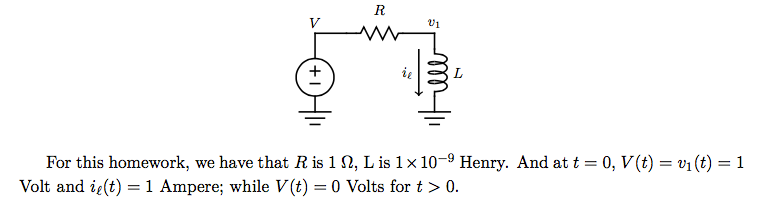
\includegraphics[width=0.9\textwidth]{./circuit.png}
 
\end{figure}

\section{Implementation: Three ODE methods}
 For this circuit, we have $$\frac{di(t)}{dt} = \frac{V(t)-R*i(t)}{L} = f(t,i(t))$$ as the system equation.\\
p. 123, and p.~123 or p.123
\begin{equation}
\abs{\frac 1 2} |\frac 1 2|
\end{equation}
\begin{equation}\label{rty}
\frac{1}{\sqrt{2\pi}}\int_1^\infty \frac 1 x  dx\\
\frac{1}{\sqrt{2\pi}}\int_1^\infty \frac 1 x \, dx
\quad \text{is divergent}
\end{equation}
\noindent By applying Forward Euler method\ref{rty}, which\eqref{rty} is $$i(t+h) = i(t) + h * f(t,i(t))$$ we have $$i(t+h) = i(t) + \frac{h(V(t)-R*i(t))}{L}$$



By applying Backward Euler method, which is $$i(t+h) = i(t) + h * f(t+h,i(t+h))$$ we have $$(1 + \frac{hR}{L}) * i(t+h) = i(t) + \frac{hV(t)}{L}$$
By applying Trapezoidal method, which is$$i(t+h) = i(t) + h * \frac{f(t,i(t)) + f(t+h,i(t+h))}{2}$$ we have $$(1 + \frac{hR}{2L}) * i(t+h) = i(t) + \frac{hV(t)}{L} - \frac{hR*i(t)}{2L}$$
As for analytical function for $i(t)$, it can be solved as $i(t) = e^{-\frac{R}{L}t}$
\section{Workflow}
\begin{description}  
\item [Usage:] ./hw13.out  $\delta$, where $\delta$ specifies different method, 1 for Forward Euler, 2 for Backward Euler, 3 for Trapezoidal Method. For example,  ./hw13.out  1 
\item [Solve:] One of the three methods is applied.
\item[Desired output:] The program can generate three different files, which are "data*.csv", "*" corresponds to the three methods mentioned above. The format of the csv file is as follow: Time, value using the specific method, analytical value, error.

\end{description}
{\bf{Notice:}} In the program, I am not able to print out specifically the value when t = $10^{-9}$ etc,. I suspect the reason is that the computer can not discern such precise accuracy.
\section{Result and Plots}
\begin{center}
\captionof{table}{Current}
\begin{tabular}{|c|c|c|c|c|}
\hline  Time(s) & Forward Euler(A)  & Backward Euler(A) & Trapezoidal(A) & Analytical(A) \\
\hline    0    	&  1	& 1 &  1 &1\\
\hline    1E-9 &   0.36417  & 0.371528 &  0.366648 	&0.367879\\
\hline    2E-9 &  0.13262	& 0.138033 &    0.134431 	&0.135335\\
\hline    3E-9 &   0.048296  &  0.051283&   0.049289	&0.049787\\
\hline    4E-9 &  0.017588	& 0.019053 &   0.018072   &0.018316\\
\hline    5E-9 &   0.006405  & 0.007079 &  0.006626 	&0.006738\\\hline 
\end{tabular}
\end{center}

\newpage
\begin{figure}[h!]
  \centering
     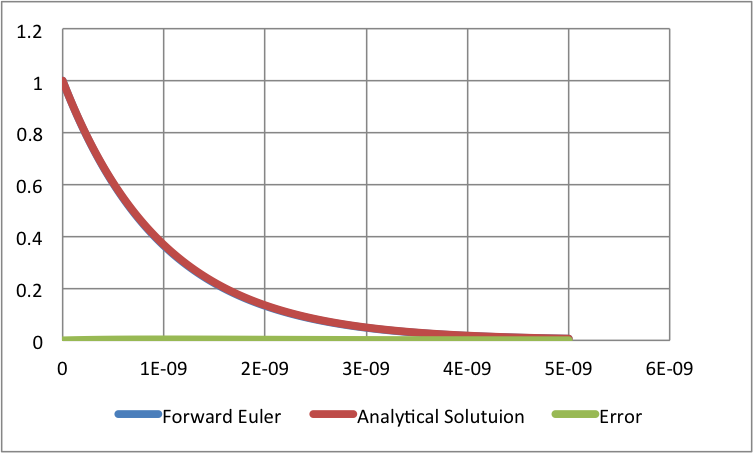
\includegraphics[width=0.9\textwidth]{./forward.png}
  \caption{Forward Euler Method I(A)-t(s) Plot}
\end{figure}

\begin{figure}[h!]
  \centering
     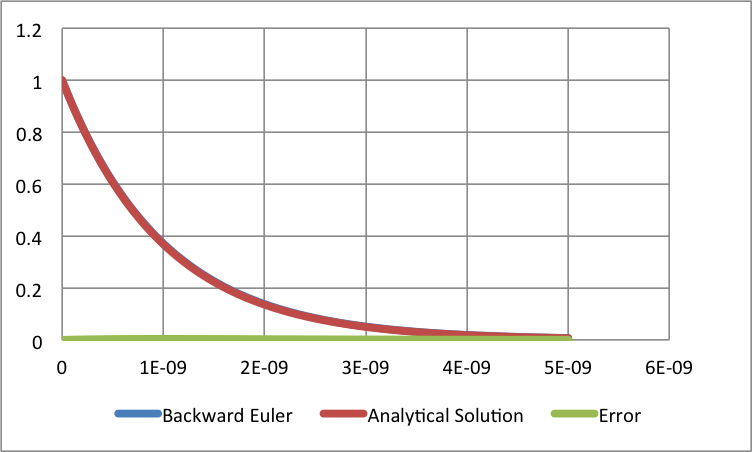
\includegraphics[width=0.9\textwidth]{./backward.png}
  \caption{Backward Euler Method I(A)-t(s) Plot}
\end{figure}


\begin{figure}[h!]
  \centering
     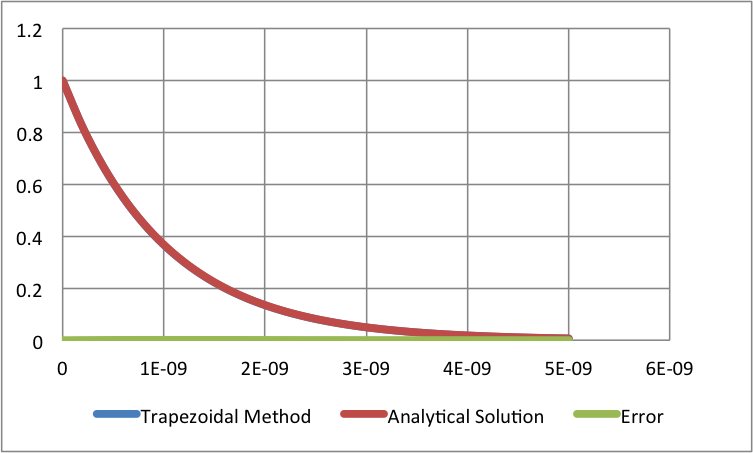
\includegraphics[width=0.9\textwidth]{./trapezoidal.png}
  \caption{Trapezoidal Method I(A)-t(s) Plot}
\end{figure}

\begin{figure}[h!]
  \centering
     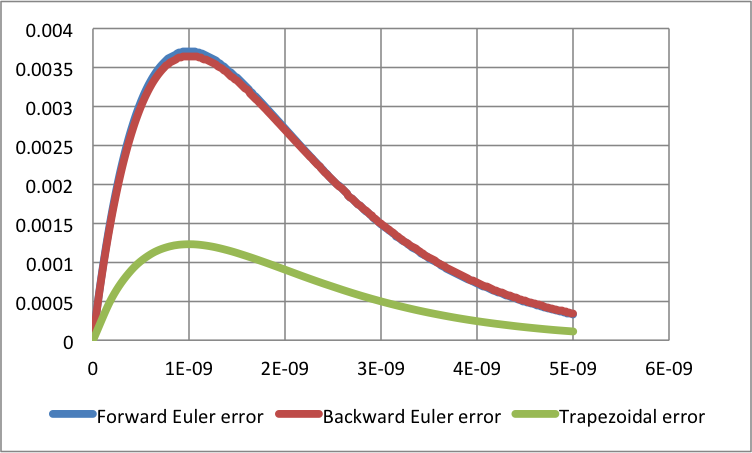
\includegraphics[width=0.9\textwidth]{./error.png}
  \caption{Error  value-t(s) Plot}
\end{figure}



\section{Observations}

As mentioned in lecture note, trapezoidal method is much more accurate than both Forward and Backward Euler method. Normally, the numerical value of Forward method is less than real value, and that of Backward method is higher than the analytical value. In sum, we can see that the error tends to converge for all three methods in the end as time is after $10^{-9}(s)$

\end{document} 
